\documentclass[landscape]{foils}
\usepackage{graphicx,color,amsmath,amssymb,latexsym,enumerate}

\topmargin-2cm
\leftmargin-1cm
%%\voffset-1.5cm
%%\hoffset.5cm
%\textwidth25cm
%\parindent0pt
\textheight18cm

\MyLogo{Ehrhart Polynomials \quad 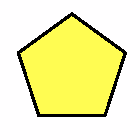
\includegraphics[viewport= 0 16 100 100, height=16pt]{pentagon} \ Matthias Beck}
\leftheader{}
\rightheader{}

\def\MB{M\hspace{-6pt}B }
\def\mybullet{\green $\blacktriangleright$ \black}

\newcounter{frozenpage}
\def\freezepage{
  \setcounter{frozenpage}{\thepage}
  \renewcommand{\thepage}{\thefrozenpage}
}
\def\thawpage{
  \count0=\thefrozenpage
  \advance\count0by1
  \renewcommand{\thepage}{\the\count0}
}

\definecolor{green}{rgb}{.0,.5,.2}             % green is not always easy to read!
\def\green{\color{green}}
\definecolor{red}{rgb}{.8,.1,.3}
\def\red{\color{red}}
\definecolor{blue}{rgb}{0,0,.7}
\def\blue{\color{blue}}
\def\black{\color{black}}
\def\yellow{\color{yellow}}
\def\cyan{\color{cyan}}
\definecolor{orange}{rgb}{1,.6,0}
\def\orange{\color{orange}}
%\def\magenta{\color{magenta}}

%\def\red{\color{black}}                       % For emergencies 
%\def\green{\color{black}}

\def\bm{\blue $} 
\def\em{$ \black } 
\def\be{\blue \[} 
\def\ee{\] \black}                               % Math mode delimiters
\def\ba{\blue \begin{eqnarray*}} 
\def\ea{\end{eqnarray*} \black}

\def\x{{\boldsymbol x}}
\def\a{{\boldsymbol a}}
\def\b{{\boldsymbol b}}
\def\p{{\boldsymbol p}}
\def\q{{\boldsymbol q}}
\def\c{c}
\DeclareMathOperator{\U}{U}

\begin{document}
\setlength{\parindent}{0pt}
\setlength{\parskip}{1cm}

\def\Z{\mathbb{Z}}
\def\Q{\mathbb{Q}}
\def\R{\mathbb{R}}
\def\F{\mathcal{F}}
\def\G{\mathcal{G}}
\def\P{\mathcal{P}}
\def\K{\mathcal{K}}
\def\cZ{\mathcal{Z}}
\def\m{\mathbf{m}}
\def\v{\mathbf{v}}
\def\w{\mathbf{w}}
\def\z{\mathbf{z}}
\newcommand\cone{\operatorname{cone}} 
\newcommand\conv{\operatorname{conv}} 
\newcommand\vol{\operatorname{vol}} 
\newcommand\stir{\operatorname{stirl}}
\newcommand\Ehr{\operatorname{Ehr}} 
\newcommand\fl[1]{\left\lfloor {#1} \right\rfloor} 
\newcommand\fr[1]{\left\{ {#1} \right\}} 

%%%%%%%%%%%%%%%%%%%%%%%%%%%%%%%%%%%%%%%%%%%%%%%%%%%%%

\thispagestyle{empty}
\

\begin{center}
  {\green\LARGE \textbf{Ehrhart Polynomials} \\[12pt]
\normalsize
Day I: Appetizers}
\end{center}

\vspace{-.2in}
%\hspace{5.3in}
\includegraphics[totalheight=5in]{../../David/sublattice3-eps-converted-to}

\vspace{-4.5in} 
\blue
\hspace{5in}
Matthias Beck
\\[5pt]
\black
\hspace{5in}
San Francisco State University
\\[5pt]
\blue
\hspace{5in}
https://matthbeck.github.io/
\black

\vspace{1in} 
\hspace{5in}
VIII Encuentro Colombiano 

\vspace{-.4in} 
\hspace{5in}
De Combinatoria

\black

%%%%%%%%%%%%%%%%%%%%%%%%%%%%%%%%%%%%%%%%%%%%%%%%%%%%%
\newpage
\[  \] 

\vspace{1.5cm} 

``Science is what we understand well enough to explain to a computer, art is all the rest." \\ 

\blue       
Donald Knuth 
\black 

\vspace{-.7in}
\hspace{5in}
\includegraphics[totalheight=3.5in]{../../David/trunccube_arrows-eps-converted-to}

%%%%%%%%%%%%%%%%%%%%%%%%%%%%%%%%%%%%%%%%%%%%%%%%%%%%%

\foilhead[-0pt]{\green Themes}

\blue
\begin{center}
Discrete-geometric \\ polynomials

\vspace{1in}
Generating \\ functions

\vspace{1in}
Polyhedra
\end{center}

\black
\vspace{-1.8in}
Combinatorial \\ structures

\vspace{-3.8in}
\hspace{7in}
Computation 

\vspace{-.4in}
\hspace{7in}
(complexity)

\vspace{-2.2in}
\hspace{-.7in}
\includegraphics[totalheight=2.8in]{../../David/permutahedron4-eps-converted-to}

\vspace{-.1in}
\hspace{6.2in}
\includegraphics[totalheight=3in]{../../David/titlepicturenolables-eps-converted-to}

%%%%%%%%%%%%%%%%%%%%%%%%%%%%%%%%%%%%%%%%%%%%%%%%%%%%%

\foilhead[-40pt]{\green A Sample Problem: Birkhoff--von Neumann Polytope}

\hspace{-.3in}
\includegraphics[totalheight=4.8in]{../oeis}

\vspace{-.7in}
\be B_n \, = \, \left\{ \left( \begin{array}{ccc} x_{11} & \cdots & x_{1n} \\ \vdots & & \vdots \\ x_{n1} & \dots & x_{nn} \end{array} \right) \in \R_{ \geq 0 }^{n^2} \, : \, \begin{array}{l} \sum_j x_{jk} = 1 \text{ for all } 1 \leq k \leq n \\ \sum_k x_{jk} = 1 \text{ for all } 1 \leq j \leq n \end{array} \right\}  \ee 

%%%%%%%%%%%%%%%%%%%%%%%%%%%%%%%%%%%%%%%%%%%%%%%%%%%%%

\foilhead[-20pt]{\green Discrete Volumes}

\red Rational polyhedron \bm \P \subset \R^d \em -- solution set of a system of linear equalities \& inequalities with integer coefficients

\green Goal: \black understand \bm \P \cap \Z^d \em \dots

\vspace{-1in}
\hspace{6.3in}
\includegraphics[totalheight=2in]{../../David/preface_disc-eps-converted-to}

\vspace{-1.5in}
\begin{enumerate}[\mybullet]
\item (list) \bm \displaystyle \sum_{ \m \in \P \cap \Z^d } z_1^{ m_1 } z_2^{ m_2 } \cdots z_d^{ m_d } \em
\item (count) \ \bm \left| \P \cap \Z^d \right| \em
\item (volume) \ \bm \displaystyle \vol(\P) \, = \, \lim_{ t \to \infty } \frac{ 1 }{ t^d } \left| \P \cap \frac 1 t \Z^d \right| \em
\end{enumerate}

\vspace{-2in}
\hspace{6.3in}
\includegraphics[totalheight=2in]{../../David/preface_cont-eps-converted-to}

\freezepage
%%%%%%%%%%%%%%%%%%%%%%%%%%%%%%%%%%%%%%%%%%%%%%%%%%%%%

\foilhead[-20pt]{\green Discrete Volumes}

\red Rational polyhedron \bm \P \subset \R^d \em -- solution set of a system of linear equalities \& inequalities with integer coefficients

\green Goal: \black understand \bm \P \cap \Z^d \em \dots

\vspace{-1in}
\hspace{6.3in}
\includegraphics[totalheight=2in]{../../David/preface_disc-eps-converted-to}

\vspace{-1.5in}
\begin{enumerate}[\mybullet]
\item (list) \bm \displaystyle \sum_{ \m \in \P \cap \Z^d } z_1^{ m_1 } z_2^{ m_2 } \cdots z_d^{ m_d } \em
\item (count) \ \bm \left| \P \cap \Z^d \right| \em
\item (volume) \ \bm \displaystyle \vol(\P) \, = \, \lim_{ t \to \infty } \frac{ 1 }{ t^d } \left| \P \cap \frac 1 t \Z^d \right| \em
\end{enumerate}

\vspace{-2in}
\hspace{6.3in}
\includegraphics[totalheight=2in]{../../David/preface_cont-eps-converted-to}

\vspace{-.2in}
\red Ehrhart function \ \bm \displaystyle L_\P (t) \, := \, \left| \P \cap \frac 1 t \Z^d \right| \, = \, \left| t \P \cap \Z^d \right| \em \ for \bm t \in \Z_{ >0 } \em

%%%%%%%%%%%%%%%%%%%%%%%%%%%%%%%%%%%%%%%%%%%%%%%%%%%%%

\foilhead[-20pt]{\green Some Motivation}

\begin{enumerate}[\mybullet]
\item Linear systems are \blue everywhere \black \!\!, and so polyhedra are everywhere.
\end{enumerate}

\thawpage
\freezepage
%%%%%%%%%%%%%%%%%%%%%%%%%%%%%%%%%%%%%%%%%%%%%%%%%%%%%

\foilhead[-20pt]{\green Some Motivation}

\begin{enumerate}[\mybullet]
\item Linear systems are \blue everywhere \black \!\!, and so polyhedra are everywhere.
\item In applications, the \blue volume \black of the polytope represented by a linear system measures some fundamental data of this system (``average").
\end{enumerate}

%%%%%%%%%%%%%%%%%%%%%%%%%%%%%%%%%%%%%%%%%%%%%%%%%%%%%

\foilhead[-20pt]{\green Some Motivation}

\begin{enumerate}[\mybullet]
\item Linear systems are \blue everywhere \black \!\!, and so polyhedra are everywhere.
\item In applications, the \blue volume \black of the polytope represented by a linear system measures some fundamental data of this system (``average").
\item Many \blue discrete problems \black in various areas are linear problems, thus they ask for the discrete volume of a polytope in disguise.
\end{enumerate}

%%%%%%%%%%%%%%%%%%%%%%%%%%%%%%%%%%%%%%%%%%%%%%%%%%%%%

\foilhead[-20pt]{\green Some Motivation}

\begin{enumerate}[\mybullet]
\item Linear systems are \blue everywhere \black \!\!, and so polyhedra are everywhere.
\item In applications, the \blue volume \black of the polytope represented by a linear system measures some fundamental data of this system (``average").
\item Many \blue discrete problems \black in various areas are linear problems, thus they ask for the discrete volume of a polytope in disguise.
\item Much discrete geometry can be modeled using \blue polynomials \black and, conversely, many combinatorial polynomials can be modeled geometrically.
\end{enumerate}

%%%%%%%%%%%%%%%%%%%%%%%%%%%%%%%%%%%%%%%%%%%%%%%%%%%%%

\foilhead[-20pt]{\green Some Motivation}

\begin{enumerate}[\mybullet]
\item Linear systems are \blue everywhere \black \!\!, and so polyhedra are everywhere.
\item In applications, the \blue volume \black of the polytope represented by a linear system measures some fundamental data of this system (``average").
\item Many \blue discrete problems \black in various areas are linear problems, thus they ask for the discrete volume of a polytope in disguise.
\item Much discrete geometry can be modeled using \blue polynomials \black and, conversely, many combinatorial polynomials can be modeled geometrically.
\item Polytopes are basic geometric objects, yet even for these basic objects volume computation is \blue hard \black and there remain many open problems.
\end{enumerate}

%%%%%%%%%%%%%%%%%%%%%%%%%%%%%%%%%%%%%%%%%%%%%%%%%%%%%

\foilhead[-20pt]{\green Some Motivation}

\begin{enumerate}[\mybullet]
\item Linear systems are \blue everywhere \black \!\!, and so polyhedra are everywhere.
\item In applications, the \blue volume \black of the polytope represented by a linear system measures some fundamental data of this system (``average").
\item Many \blue discrete problems \black in various areas are linear problems, thus they ask for the discrete volume of a polytope in disguise.
\item Much discrete geometry can be modeled using \blue polynomials \black and, conversely, many combinatorial polynomials can be modeled geometrically.
\item Polytopes are basic geometric objects, yet even for these basic objects volume computation is \blue hard \black and there remain many open problems.
\item Also, polytopes are \blue cool \black\!\!.
\end{enumerate}

%%%%%%%%%%%%%%%%%%%%%%%%%%%%%%%%%%%%%%%%%%%%%%%%%%%%%

\foilhead{\green Today's Menu: Get Our Hands Dirty}

\vspace{-.3in}
\hspace{2.3in}
\includegraphics[totalheight=3in]{../../David/cube-eps-converted-to}

\vspace{-1.6in}
%\hspace{3in}
%\includegraphics[totalheight=3in]{../../David/standsimplex-eps-converted-to}
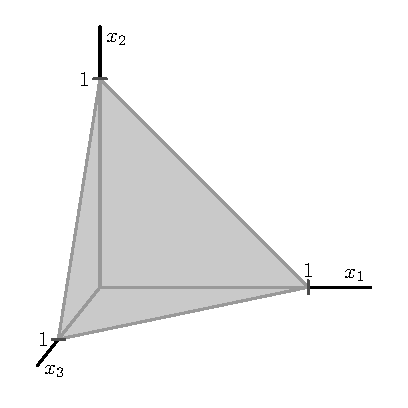
\includegraphics[totalheight=4in]{../../David/fig22c}

\vspace{-4.3in}
\hspace{5in}
\includegraphics[totalheight=4.2in]{../../David/octahedron-eps-converted-to}

\thawpage
%%%%%%%%%%%%%%%%%%%%%%%%%%%%%%%%%%%%%%%%%%%%%%%%%%%%%

\foilhead[-20pt]{\green The Unit Cube}

\red Lattice polytope \bm \P \subset \R^d \em -- convex hull of finitely points in \bm \Z^d \em

For \bm t \in \Z_{ >0 } \em let \bm L_\P (t) \, := \, \# \left( t \P \cap \Z^d \right) \em

The \red unit cube \black in \bm \R^d \em is
\ \bm \P \, = \, [0,1]^d \, = \, \left\{ \x \in \R^d : \, 0 \le x_j \le 1 \right\}  \em

\vspace{.1in}
%\hspace{4.3in}
\includegraphics[totalheight=3.4in]{../../David/cube-eps-converted-to}

\vspace{-3.3in}
\hspace{4.3in}
\green $\longrightarrow$ \ \bm L_\P(t) \, = \, (t+1)^d \em

\freezepage
%%%%%%%%%%%%%%%%%%%%%%%%%%%%%%%%%%%%%%%%%%%%%%%%%%%%%

\foilhead[-20pt]{\green The Unit Cube}

\red Lattice polytope \bm \P \subset \R^d \em -- convex hull of finitely points in \bm \Z^d \em

For \bm t \in \Z_{ >0 } \em let \bm L_\P (t) \, := \, \# \left( t \P \cap \Z^d \right) \em

The \red unit cube \black in \bm \R^d \em is
\ \bm \P \, = \, [0,1]^d \, = \, \left\{ \x \in \R^d : \, 0 \le x_j \le 1 \right\}  \em

\vspace{.1in}
%\hspace{4.3in}
\includegraphics[totalheight=3.4in]{../../David/cube-eps-converted-to}

\vspace{-3.3in}
\hspace{4.3in}
\green $\longrightarrow$ \ \bm L_\P(t) \, = \, (t+1)^d \em

\vspace{.6in}
\hspace{4.82in}
\green \bm L_{\P^\circ}(t) \, = \, (t-1)^d \em

%%%%%%%%%%%%%%%%%%%%%%%%%%%%%%%%%%%%%%%%%%%%%%%%%%%%%

\foilhead[-20pt]{\green The Standard Simplex}

The \red standard simplex \bm \Delta \in \R^d \em is the convex hull of the
unit vectors and the origin; alternatively,

\vspace{.3in}
\hspace{2.9in}
\bm
\Delta \ = \ \left\{ \x \in \R_{ \ge 0 }^d : \, x_1 + x_2 + \cdots + x_d \le 1 \right\}
\em

\vspace{-.6in}
%\hspace{.3in}
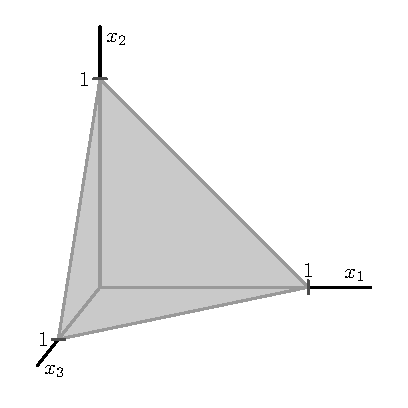
\includegraphics[totalheight=4in]{../../David/fig22c}

\thawpage
\freezepage
%%%%%%%%%%%%%%%%%%%%%%%%%%%%%%%%%%%%%%%%%%%%%%%%%%%%%

\foilhead[-20pt]{\green The Standard Simplex}

The \red standard simplex \bm \Delta \in \R^d \em is the convex hull of the
unit vectors and the origin; alternatively,
\be
\Delta \ = \ \left\{ \x \in \R_{ \ge 0 }^d : \, x_1 + x_2 + \cdots + x_d \le 1 \right\}
\ee

\vspace{-1in}
\ba
L_\Delta(t) 
&=& \# \left\{ (x_1, x_2 \dots, x_d) \in \Z_{ \ge 0 }^d : \, x_1 + x_2 + \cdots + x_d \le t \right\} \\
&=& \# \left\{ (x_1, x_2 \dots, x_d, x_{ d+1 } ) \in \Z_{ \ge 0 }^{d+1} : \, x_1 +
x_2 + \cdots + x_{ d+1 } = t \right\} \\
&=& \binom{ d+t } d
\ea

%%%%%%%%%%%%%%%%%%%%%%%%%%%%%%%%%%%%%%%%%%%%%%%%%%%%%

\foilhead[-20pt]{\green The Standard Simplex}

The \red standard simplex \bm \Delta \in \R^d \em is the convex hull of the
unit vectors and the origin; alternatively,
\be
\Delta \ = \ \left\{ (x_1, x_2 \dots, x_d) \in \R_{ \ge 0 }^d : \, x_1 + x_2 + \cdots + x_d \le 1 \right\}
\ee

\vspace{-1in}
\ba
L_\Delta(t) 
&=& \# \left\{ (x_1, x_2 \dots, x_d) \in \Z_{ \ge 0 }^d : \, x_1 + x_2 + \cdots + x_d \le t \right\} \\
&=& \# \left\{ (x_1, x_2 \dots, x_d, x_{ d+1 } ) \in \Z_{ \ge 0 }^{d+1} : \, x_1 +
x_2 + \cdots + x_{ d+1 } = t \right\} \\
&=& \binom{ d+t } d
\ea

\vspace{-.2in}
\bm \displaystyle
L_{ \Delta^\circ } (t) \ = \ \binom{t-1} d 
\em

%%%%%%%%%%%%%%%%%%%%%%%%%%%%%%%%%%%%%%%%%%%%%%%%%%%%%

\foilhead[-20pt]{\green The Cross-Polytope}

The \red cross-polytope \bm \Diamond \in \R^d \em is

\bm
\Diamond \ = \ \left\{ \x \in \R^d : \, \left| x_1 \right| + \left| x_2 \right| + \dots + \left| x_d \right| \leq 1 \right\}
\em

\vspace{-1.7in}
\hspace{5in}
\includegraphics[totalheight=3.9in]{../../David/octahedron-eps-converted-to}

\thawpage
\freezepage
%%%%%%%%%%%%%%%%%%%%%%%%%%%%%%%%%%%%%%%%%%%%%%%%%%%%%

\foilhead[-20pt]{\green The Cross-Polytope}

The \red cross-polytope \bm \Diamond \in \R^d \em is

\bm
\Diamond \ = \ \left\{ \x \in \R^d : \, \left| x_1 \right| + \left| x_2 \right| + \dots + \left| x_d \right| \leq 1 \right\}
\em

\vspace{-1.7in}
\hspace{5in}
\includegraphics[totalheight=3.9in]{../../David/octahedron-eps-converted-to}

\vspace{-2.3in}
Let's compute \bm L_\Diamond(t) \em for \bm d=3 \em \dots

\vspace{.2in}
\begin{enumerate}[\mybullet]
\item Triangulation
\item Disjoint triangulation
\item Interpolation
\item Generating function
\end{enumerate}

%%%%%%%%%%%%%%%%%%%%%%%%%%%%%%%%%%%%%%%%%%%%%%%%%%%%%

\foilhead[-20pt]{\green The Cross-Polytope}

The \red cross-polytope \bm \Diamond \in \R^d \em is

\bm
\Diamond \ = \ \left\{ \x \in \R^d : \, \left| x_1 \right| + \left| x_2 \right| + \dots + \left| x_d \right| \leq 1 \right\}
\em

\vspace{-1.7in}
\hspace{5in}
\includegraphics[totalheight=3.9in]{../../David/octahedron-eps-converted-to}

\vspace{-2.3in}
Let's compute \bm L_\Diamond(t) \em for \bm d=3 \em \dots

\vspace{.2in}
\begin{enumerate}[\mybullet]
\item Triangulation
\end{enumerate}

Dissect \bm \Diamond \em into \bm 8 \em (standard) tetrahedra and use
inclusion--exclusion to compute \bm L_\Diamond(t) \em

%%%%%%%%%%%%%%%%%%%%%%%%%%%%%%%%%%%%%%%%%%%%%%%%%%%%%

\foilhead[-20pt]{\green The Cross-Polytope}

The \red cross-polytope \bm \Diamond \in \R^d \em is

\bm
\Diamond \ = \ \left\{ \x \in \R^d : \, \left| x_1 \right| + \left| x_2 \right| + \dots + \left| x_d \right| \leq 1 \right\}
\em

\vspace{-1.7in}
\hspace{5in}
\includegraphics[totalheight=3.9in]{../../David/octahedron-eps-converted-to}

\vspace{-2.3in}
Let's compute \bm L_\Diamond(t) \em for \bm d=3 \em \dots

\vspace{.2in}
\begin{enumerate}[\mybullet]
\item Disjoint triangulation
\end{enumerate}

Dissect \bm \Diamond \em into \bm 8 \em half-open tetrahedra 

%%%%%%%%%%%%%%%%%%%%%%%%%%%%%%%%%%%%%%%%%%%%%%%%%%%%%

\foilhead[-20pt]{\green The Cross-Polytope}

The \red cross-polytope \bm \Diamond \in \R^d \em is

\bm
\Diamond \ = \ \left\{ \x \in \R^d : \, \left| x_1 \right| + \left| x_2 \right| + \dots + \left| x_d \right| \leq 1 \right\}
\em

\vspace{-1.7in}
\hspace{5in}
\includegraphics[totalheight=3.9in]{../../David/octahedron-eps-converted-to}

\vspace{-2.3in}
Let's compute \bm L_\Diamond(t) \em for \bm d=3 \em \dots

\vspace{-.1in}
\begin{enumerate}[\mybullet]
\item Interpolation
\end{enumerate}

\vspace{-.1in}
%\hspace{2.3in}
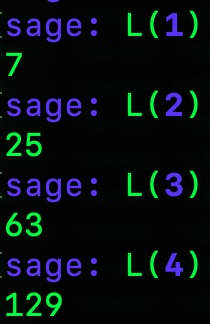
\includegraphics[totalheight=2.3in]{interpol}

% V = matrix.vandermonde([1,2,3,4])

\thawpage
%%%%%%%%%%%%%%%%%%%%%%%%%%%%%%%%%%%%%%%%%%%%%%%%%%%%%

\foilhead[-20pt]{\green The Cross-Polytope}

The \red cross-polytope \bm \Diamond \in \R^d \em is

\bm
\Diamond \ = \ \left\{ \x \in \R^d : \, \left| x_1 \right| + \left| x_2 \right| + \dots + \left| x_d \right| \leq 1 \right\}
\em

\vspace{-1.7in}
\hspace{5in}
\includegraphics[totalheight=3.9in]{../../David/octahedron-eps-converted-to}

\vspace{-2.3in}
Let's compute \bm L_\Diamond(t) \em for \bm d=3 \em \dots

\vspace{.2in}
\begin{enumerate}[\mybullet]
\item Generating function
\end{enumerate}

\vspace{-.4in}
\hspace{3in}
\bm \displaystyle \Ehr_\P (z) \, := \, 1 + \sum_{ t \ge 1 } L_\P (t) \, z^t \em 

\vspace{-.1in}
Exercise:
\newcommand\DouPyr{\operatorname{BiPyr}} 
\bm \displaystyle
\Ehr_{ \DouPyr (\P) } (z) \ = \ \frac{ 1+z }{ 1-z } \Ehr_\P (z) 
\em

\vspace{.1in}
\hspace{3.5in}
\dots for unit cubes \ \green $\longrightarrow$ \ \black Eulerian polynomials

%%%%%%%%%%%%%%%%%%%%%%%%%%%%%%%%%%%%%%%%%%%%%%%%%%%%%

\foilhead{\green Zonotopes}

\vspace{-1.4in}
\hspace{7in}
\includegraphics[totalheight=2.2in]{../../David/trunccube_arrows-eps-converted-to}

\vspace{-1.4in}
Line segment \
\bm [\a,\b] := \{ (1-\lambda) \, \a + \lambda \, \b : \, 0 \le \lambda \le 1 \} \em

Minkowski sum \
\bm \K_1 + \K_2 \ := \ \{ \p+\q : \, \p \in \K_1, \ \q \in \K_2 \} \em 

\hspace{2.5in}
Zonotope \ \bm \cZ := [\a_1,\b_1] + [\a_2,\b_2] + \cdots + [\a_m,\b_m] \em

\vspace{-.9in}
\includegraphics[totalheight=2.2in]{../../David/zonotopeex-eps-converted-to}

\freezepage
%%%%%%%%%%%%%%%%%%%%%%%%%%%%%%%%%%%%%%%%%%%%%%%%%%%%%

\foilhead{\green Zonotopes}

\vspace{-1.4in}
\hspace{7in}
\includegraphics[totalheight=2.2in]{../../David/trunccube_arrows-eps-converted-to}

\vspace{-1.4in}
Line segment \
\bm [\a,\b] := \{ (1-\lambda) \, \a + \lambda \, \b : \, 0 \le \lambda \le 1 \} \em

Minkowski sum \
\bm \K_1 + \K_2 \ := \ \{ \p+\q : \, \p \in \K_1, \ \q \in \K_2 \} \em 

\hspace{2.5in}
Zonotope \ \bm \cZ := [\a_1,\b_1] + [\a_2,\b_2] + \cdots + [\a_m,\b_m] \em

\vspace{-.9in}
\includegraphics[totalheight=2.2in]{../../David/zonotopeex-eps-converted-to}

\vspace{-1.8in}
\hspace{2.5in}
Every zonotope admits a \red tiling \black into parallelepipeds

\vspace{-.3in}
\hspace{4.1in}
\includegraphics[totalheight=3in]{../../David/zonotopepaving-eps-converted-to}

\vspace{-1.8in}
\bm \P \em --- half-open \bm d \em\!\!-parallelepiped

\green $\longrightarrow$ \ \bm L_\P(t) \, = \, t^d \em

%%%%%%%%%%%%%%%%%%%%%%%%%%%%%%%%%%%%%%%%%%%%%%%%%%%%%

\foilhead{\green Birkhoff--von Neumann Revisited}

\vspace{-.7in}
\includegraphics[totalheight=5.8in]{../birkhoff9roots}

\vspace{-4.5in}
\hspace{5in}
For more about roots of 

\vspace{-.35in}
\hspace{5in}
(Ehrhart) polynomials, 

\vspace{-.35in}
\hspace{5in}
see Braun (2008) and 

\vspace{-.35in}
\hspace{5in}
Pfeifle (2010).

\thawpage
%%%%%%%%%%%%%%%%%%%%%%%%%%%%%%%%%%%%%%%%%%%%%%%%%%%%%

\foilhead{\green Recap Day I}

\vspace{-.2in}
\begin{enumerate}[\mybullet]
\item Volume computations \ \bm \longrightarrow \em \ don't agonize, discretize 
\item Integer-point counting in dilated polytopes \ \bm \longrightarrow \em \
polynomials
\item Interpolation
\item Generating functions
\item Dissections: triangulations, tilings
\item Tomorrow: enough practice, how \\ does this work in theory?
\end{enumerate}

\vspace{-3.2in}
\hspace{5.7in}
\includegraphics[totalheight=3.5in]{../../David/truncsmallicos_arrows-eps-converted-to}

%%%%%%%%%%%%%%%%%%%%%%%%%%%%%%%%%%%%%%%%%%%%%%%%%%%%%

% \end{document}

%%%%%%%%%%%%%%%%%%%%%%%%%%%%%%%%%%%%%%%%%%%%%%%%%%%%%

\newpage
\thispagestyle{empty}
\

\begin{center}
  {\green\LARGE \textbf{Ehrhart Polynomials} \\[12pt]
\normalsize
Day II: Generating Functions \& Complexity}
\end{center}

\vspace{-.2in}
%\hspace{5.3in}
\includegraphics[totalheight=5in]{../../David/sublattice3-eps-converted-to}

\vspace{-4.5in} 
\blue
\hspace{5in}
Matthias Beck
\\[5pt]
\black
\hspace{5in}
San Francisco State University
\\[5pt]
\blue
\hspace{5in}
https://matthbeck.github.io/
\black

\vspace{1in} 
\hspace{5in}
VIII Encuentro Colombiano 

\vspace{-.4in} 
\hspace{5in}
De Combinatoria

\black

\setcounter{page}{1}

%%%%%%%%%%%%%%%%%%%%%%%%%%%%%%%%%%%%%%%%%%%%%%%%%%%%%

\foilhead{\green Any questions about yesterday?}

\vspace{-.1in}
\hspace{4.3in}
\includegraphics[totalheight=2in]{../../David/preface_disc-eps-converted-to}
\hspace{-.1in}
\includegraphics[totalheight=2in]{../../David/preface_cont-eps-converted-to}

\vspace{-2.9in}
\includegraphics[totalheight=3.3in]{../../David/octahedron-eps-converted-to}

\vspace{-.5in}
\includegraphics[totalheight=3in]{../../David/zonotopepaving-eps-converted-to}

\vspace{-3.3in}
\hspace{6in}
\includegraphics[totalheight=3in]{../../David/trunccube_arrows-eps-converted-to}

%%%%%%%%%%%%%%%%%%%%%%%%%%%%%%%%%%%%%%%%%%%%%%%%%%%%%

\foilhead[-20pt]{\green Warm-Up: Partition Generating Functions}

A \red partition \bm \lambda = \left( \lambda_1, \lambda_2, \dots, \lambda_n \right) \em of an integer \bm k \ge 0 \em satisfies
\be
  k = \lambda_1 + \lambda_2 + \dots + \lambda_n
  \qquad \text{ \black and } \qquad
  0 \le \lambda_1 \le \lambda_2 \le \dots \le \lambda_n
\ee
\red Goal \ \black Compute \
% \bm \displaystyle \sum_{ \lambda } x_1^{ \lambda_1 } \cdots x_n^{ \lambda_n } \em \ or \
\bm \displaystyle \sum_{ \lambda } q^{ \lambda_1 + \dots + \lambda_n } \em 
% where the sums run through your favorite partitions.
over your favorite partition family

\red Example \black \ \bm P_{ \le 3 } \em --- family of partitions into at most \bm 3 \em parts
\be
  \sum_{ \lambda \in P_{ \le 3 } } q^{ \lambda_1 + \lambda_2 + \lambda_3 } \ = \ \frac{ 1 }{ (1-q) (1-q^2) (1-q^3) } 
\ee

\freezepage
%%%%%%%%%%%%%%%%%%%%%%%%%%%%%%%%%%%%%%%%%%%%%%%%%%%%%

\foilhead[-20pt]{\green Warm-Up: Partition Generating Functions}

A \red partition \bm \lambda = \left( \lambda_1, \lambda_2, \dots, \lambda_n \right) \em of an integer \bm k \ge 0 \em satisfies
\be
  k = \lambda_1 + \lambda_2 + \dots + \lambda_n
  \qquad \text{ \black and } \qquad
  0 \le \lambda_1 \le \lambda_2 \le \dots \le \lambda_n
\ee
\red Goal \ \black Compute \
% \bm \displaystyle \sum_{ \lambda } x_1^{ \lambda_1 } \cdots x_n^{ \lambda_n } \em \ or \
\bm \displaystyle \sum_{ \lambda } q^{ \lambda_1 + \dots + \lambda_n } \em 
% where the sums run through your favorite partitions.
over your favorite partition family

\red Example \black \ \bm P_{ \le 3 } \em --- family of partitions into at most \bm 3 \em parts
\be
  \sum_{ \lambda \in P_{ \le 3 } } q^{ \lambda_1 + \lambda_2 + \lambda_3 } \ = \ \frac{ 1
}{ (1-q) (1-q^2) (1-q^3) } 
\ee
\red Idea \ 
\bm P_{ \le 3 } \ = \ \left\{ \lambda \in \Z^3 : \, 0 \le \lambda_1 \le \lambda_2 \le \lambda_3 \right\} \ = \ \K \cap \Z^3 \em 

\hspace{.83in}
\bm \K \ = \ \left\{ \x \in \R^3 : \, 0 \le x_1 \le x_2 \le x_3 \right\} \em
\ \green $\longleftarrow$ \ polyhedral cone $\heartsuit$

%%%%%%%%%%%%%%%%%%%%%%%%%%%%%%%%%%%%%%%%%%%%%%%%%%%%%

\foilhead[-20pt]{\green Warm-Up: Partition Generating Functions}

\bm \K \ = \ \left\{ \x \in \R^3 : \, 0 \le x_1 \le x_2 \le x_3 \right\}
  \ = \ \R_{ \ge 0 } \begin{bmatrix} 0 \\ 0 \\ 1 \end{bmatrix} + 
  \R_{ \ge 0 } \begin{bmatrix} 0 \\ 1 \\ 1 \end{bmatrix} + 
  \R_{ \ge 0 } \begin{bmatrix} 1 \\ 1 \\ 1 \end{bmatrix} 
\em

is a rational, simplicial, unimodular cone

\vspace{-.6in}
\hspace{6in}
\bm \det \begin{bmatrix} 0 & 0 & 1 \\ 0 & 1 & 1 \\ 1 & 1 & 1 \end{bmatrix} = -1 \em

\thawpage
\freezepage
%%%%%%%%%%%%%%%%%%%%%%%%%%%%%%%%%%%%%%%%%%%%%%%%%%%%%

\foilhead[-20pt]{\green Warm-Up: Partition Generating Functions}

\bm \K \ = \ \left\{ \x \in \R^3 : \, 0 \le x_1 \le x_2 \le x_3 \right\}
  \ = \ \R_{ \ge 0 } \begin{bmatrix} 0 \\ 0 \\ 1 \end{bmatrix} + 
  \R_{ \ge 0 } \begin{bmatrix} 0 \\ 1 \\ 1 \end{bmatrix} + 
  \R_{ \ge 0 } \begin{bmatrix} 1 \\ 1 \\ 1 \end{bmatrix} 
\em

is a rational, simplicial, unimodular cone

\vspace{-.6in}
\hspace{6in}
\bm \det \begin{bmatrix} 0 & 0 & 1 \\ 0 & 1 & 1 \\ 1 & 1 & 1 \end{bmatrix} = -1 \em

\vspace{-.3in}
\red Integer-point transform
\ba
  \sigma_{ \K } (z_1, z_2, z_3)
  &=& \sum_{ \m \in \K \cap \Z^3 } z_1^{ m_1 } z_2^{ m_2 } z_3^{ m_3 } \\
  &=& \frac{ 1 }{ (1-z_3) (1-z_2 z_3) (1-z_1 z_2 z_3) } 
\ea

%%%%%%%%%%%%%%%%%%%%%%%%%%%%%%%%%%%%%%%%%%%%%%%%%%%%%

\foilhead[-20pt]{\green Warm-Up: Partition Generating Functions}

\bm \K \ = \ \left\{ \x \in \R^3 : \, 0 \le x_1 \le x_2 \le x_3 \right\}
  \ = \ \R_{ \ge 0 } \begin{bmatrix} 0 \\ 0 \\ 1 \end{bmatrix} + 
  \R_{ \ge 0 } \begin{bmatrix} 0 \\ 1 \\ 1 \end{bmatrix} + 
  \R_{ \ge 0 } \begin{bmatrix} 1 \\ 1 \\ 1 \end{bmatrix} 
\em

is a rational, simplicial, unimodular cone

\vspace{-.6in}
\hspace{6in}
\bm \det \begin{bmatrix} 0 & 0 & 1 \\ 0 & 1 & 1 \\ 1 & 1 & 1 \end{bmatrix} = -1 \em

\vspace{-.3in}
\red Integer-point transform
\ba
  \sigma_{ \K } (z_1, z_2, z_3)
  &=& \sum_{ \m \in \K \cap \Z^3 } z_1^{ m_1 } z_2^{ m_2 } z_3^{ m_3 } \\
  &=& \frac{ 1 }{ (1-z_3) (1-z_2 z_3) (1-z_1 z_2 z_3) } 
\ea
\be
  \sum_{ \lambda \in P_{ \le 3 } } q^{ \lambda_1 + \lambda_2 + \lambda_3 }
  \ = \ \sigma_{ \K } (q,q,q)
  \ = \ \frac{ 1 }{ (1-q) (1-q^2) (1-q^3) } 
\ee

%%%%%%%%%%%%%%%%%%%%%%%%%%%%%%%%%%%%%%%%%%%%%%%%%%%%%

\foilhead[-20pt]{\green Variations on a Theme}

\bm P_{ 3 } \em --- family of partitions into \red exactly \bm 3 \em parts
 
\bm P_{ 3 } \ = \ \left\{ \lambda \in \Z^3 : \, 0 < \lambda_1 \le \lambda_2 \le
\lambda_3 \right\} \ = \ \widetilde\K \cap \Z^3 \em 

\hspace{.02in}
\bm \widetilde\K \ = \ \left\{ \x \in \R^3 : \, 0 < x_1 \le x_2 \le x_3 \right\}
  \ = \ \R_{ \ge 0 } \begin{bmatrix} 0 \\ 0 \\ 1 \end{bmatrix} + 
  \R_{ \ge 0 } \begin{bmatrix} 0 \\ 1 \\ 1 \end{bmatrix} + 
  \R_{ > 0 } \begin{bmatrix} 1 \\ 1 \\ 1 \end{bmatrix}
\em

\thawpage
\freezepage
%%%%%%%%%%%%%%%%%%%%%%%%%%%%%%%%%%%%%%%%%%%%%%%%%%%%%

\foilhead[-20pt]{\green Variations on a Theme}

\bm P_{ 3 } \em --- family of partitions into \red exactly \bm 3 \em parts
 
\bm P_{ 3 } \ = \ \left\{ \lambda \in \Z^3 : \, 0 < \lambda_1 \le \lambda_2 \le
\lambda_3 \right\} \ = \ \widetilde\K \cap \Z^3 \em 

\hspace{.02in}
\bm \widetilde\K \ = \ \left\{ \x \in \R^3 : \, 0 < x_1 \le x_2 \le x_3 \right\}
  \ = \ \R_{ \ge 0 } \begin{bmatrix} 0 \\ 0 \\ 1 \end{bmatrix} + 
  \R_{ \ge 0 } \begin{bmatrix} 0 \\ 1 \\ 1 \end{bmatrix} + 
  \R_{ > 0 } \begin{bmatrix} 1 \\ 1 \\ 1 \end{bmatrix}
\em
%
\ba
  \sigma_{ \widetilde\K } (z_1, z_2, z_3)
  &=& \sum_{ \m \in \widetilde\K \cap \Z^3 } z_1^{ m_1 } z_2^{ m_2 } z_3^{ m_3 } \\
  &=& \frac{ z_1 z_2 z_3 }{ (1-z_3) (1-z_2 z_3) (1-z_1 z_2 z_3) } 
\ea
\be
  \sum_{ \lambda \in P_{ 3 } } q^{ \lambda_1 + \lambda_2 + \lambda_3 }
  \ = \ \sigma_{ \widetilde\K } (q,q,q)
  \ = \ \frac{ q^3 }{ (1-q) (1-q^2) (1-q^3) } 
\ee

%%%%%%%%%%%%%%%%%%%%%%%%%%%%%%%%%%%%%%%%%%%%%%%%%%%%%

\foilhead[-20pt]{\green Integer-point Complexity of a Simplicial Cone}

What if \bm \K \em is (still simplicial and rational but) not unimodular?
\\
Say \bm \w_1, \w_2, \w_3 \in \Z^3 \em are linearly independent,
\bm \det [\w_1 \, \w_2 \, \w_3] = D > 1 \em

\bm \K = \R_{ \ge 0 } \, \w_1 + \R_{ \ge 0 } \, \w_2 + \R_{ \ge 0 } \, \w_3 \em

\thawpage
\freezepage
%%%%%%%%%%%%%%%%%%%%%%%%%%%%%%%%%%%%%%%%%%%%%%%%%%%%%

\foilhead[-20pt]{\green Integer-point Complexity of a Simplicial Cone}

What if \bm \K \em is (still simplicial and rational but) not unimodular?
\\
Say \bm \w_1, \w_2, \w_3 \in \Z^3 \em are linearly independent,
\bm \det [\w_1 \, \w_2 \, \w_3] = D > 1 \em

\bm \K = \R_{ \ge 0 } \, \w_1 + \R_{ \ge 0 } \, \w_2 + \R_{ \ge 0 } \, \w_3 \em

\red Idea \black \ Tile \bm \K \em with the half-open parallelepiped
\\
\bm \Pi = [0,1) \, \w_1 + [0,1) \, \w_2 + [0,1) \, \w_3 \em

\vspace{-1.9in}
\hspace{5.8in}
\includegraphics[totalheight=3in]{../../../CRT-Book/David/3dim-tiling-domain}

\vspace{-1.4in}
\includegraphics[totalheight=3in]{../../../CRT-Book/David/3dim-tiling}

%%%%%%%%%%%%%%%%%%%%%%%%%%%%%%%%%%%%%%%%%%%%%%%%%%%%%

\foilhead[-20pt]{\green Integer-point Complexity of a Simplicial Cone}

What if \bm \K \em is (still simplicial and rational but) not unimodular?
\\
Say \bm \w_1, \w_2, \w_3 \in \Z^3 \em are linearly independent,
\bm \det [\w_1 \, \w_2 \, \w_3] = D > 1 \em

\bm \K = \R_{ \ge 0 } \, \w_1 + \R_{ \ge 0 } \, \w_2 + \R_{ \ge 0 } \, \w_3 \em

\red Idea \black \ Tile \bm \K \em with the half-open parallelepiped
\\
\bm \Pi = [0,1) \, \w_1 + [0,1) \, \w_2 + [0,1) \, \w_3 \em

\vspace{-1.9in}
\hspace{5.8in}
\includegraphics[totalheight=3in]{../../../CRT-Book/David/3dim-tiling-domain}

\vspace{-1.4in}
\includegraphics[totalheight=3in]{../../../CRT-Book/David/3dim-tiling}

\vspace{-3.5in}
\hspace{4.2in}
\green $\downarrow$

\hspace{3.7in}
\bm \sigma_\K(z_1, z_2, z_3) = \em

\vspace{-.2in}
\hspace{3.7in}
\bm \displaystyle \frac{ \sigma_\Pi(z_1, z_2, z_3) }{ (1 - \z^{ \w_1 }) (1 - \z^{
\w_2 }) (1 - \z^{ \w_3 })  } \em

\hspace{3.7in}
where \bm \z^\m = z_1^{ m_1 } z_2^{ m_2 } z_3^{ m_3 } \em

%%%%%%%%%%%%%%%%%%%%%%%%%%%%%%%%%%%%%%%%%%%%%%%%%%%%%

\foilhead[-20pt]{\green Integer-point Complexity of a Simplicial Cone}

What if \bm \K \em is (still simplicial and rational but) not unimodular?
\\
Say \bm \w_1, \w_2, \w_3 \in \Z^3 \em are linearly independent,
\bm \det [\w_1 \, \w_2 \, \w_3] = D > 1 \em

\bm \K = \R_{ \ge 0 } \, \w_1 + \R_{ \ge 0 } \, \w_2 + \R_{ \ge 0 } \, \w_3 \em

\red Idea \black \ Tile \bm \K \em with the half-open parallelepiped
\\
\bm \Pi = [0,1) \, \w_1 + [0,1) \, \w_2 + [0,1) \, \w_3 \em

\vspace{-1.9in}
\hspace{5.8in}
\includegraphics[totalheight=3in]{../../../CRT-Book/David/3dim-tiling-domain}

\vspace{-1.4in}
\includegraphics[totalheight=3in]{../../../CRT-Book/David/3dim-tiling}

\vspace{-3.5in}
\hspace{4.2in}
\green $\downarrow$

\hspace{3.7in}
\bm \sigma_\K(z_1, z_2, z_3) = \em

\vspace{-.2in}
\hspace{3.7in}
\bm \displaystyle \frac{ \sigma_\Pi(z_1, z_2, z_3) }{ (1 - \z^{ \w_1 }) (1 - \z^{
\w_2 }) (1 - \z^{ \w_3 })  } \em

\vspace{.2in}
\hspace{3.7in}
\red Complexity \black\!\!: \bm \sigma_\Pi(z_1, z_2, z_3) \em has \bm D \em terms

%%%%%%%%%%%%%%%%%%%%%%%%%%%%%%%%%%%%%%%%%%%%%%%%%%%%%

\foilhead[-20pt]{\green Homogenizing Polytopes}

Given a polytope \bm \P \subset \R^d \em let

\bm \cone(\P) \, := \, \R_{ \ge 0 } \left( \P \times \{ 1 \} \right) \subset \R^{
d+1 } \em

\vspace{-.2in}
\bm = \, \R_{ \ge 0 } \begin{bmatrix} \v_1 \\ 1 \end{bmatrix} 
  + \R_{ \ge 0 } \begin{bmatrix} \v_2 \\ 1 \end{bmatrix}
  + \dots + \R_{ \ge 0 } \begin{bmatrix} \v_n \\ 1 \end{bmatrix} \em

\vspace{-2.9in}
\hspace{5.2in}
\includegraphics[totalheight=4in]{../../David/titlepicturenolables-eps-converted-to}

\vspace{-1.1in}
\bm \cone(\P) \cap \{ \x \in \R^{ d+1 } : \, x_{ d+1 } = t \} \em
% = t\P \times \{ t \} \em

\vspace{-.2in}
contains a copy of \bm t\P \em 

\thawpage
\freezepage
%%%%%%%%%%%%%%%%%%%%%%%%%%%%%%%%%%%%%%%%%%%%%%%%%%%%%

\foilhead[-20pt]{\green Homogenizing Polytopes}

Given a polytope \bm \P \subset \R^d \em let

\bm \cone(\P) \, := \, \R_{ \ge 0 } \left( \P \times \{ 1 \} \right) \subset \R^{
d+1 } \em

\vspace{-.2in}
\bm = \, \R_{ \ge 0 } \begin{bmatrix} \v_1 \\ 1 \end{bmatrix} 
  + \R_{ \ge 0 } \begin{bmatrix} \v_2 \\ 1 \end{bmatrix}
  + \dots + \R_{ \ge 0 } \begin{bmatrix} \v_n \\ 1 \end{bmatrix} \em

\vspace{-2.9in}
\hspace{5.2in}
\includegraphics[totalheight=4in]{../../David/titlepicturenolables-eps-converted-to}

\vspace{-1.1in}
\bm \cone(\P) \cap \{ \x \in \R^{ d+1 } : \, x_{ d+1 } = t \} \em
% = t\P \times \{ t \} \em

\vspace{-.2in}
contains a copy of \bm t\P \em \ \green $\longrightarrow$

\vspace{-.4in}
\be \displaystyle \Ehr_\P (z) \, := \, 1 + \sum_{ t \ge 1 } L_\P (t) \, z^t 
\, = \, \sigma_{ \cone(\P) } (1, 1, \dots, 1, z) \ee

%%%%%%%%%%%%%%%%%%%%%%%%%%%%%%%%%%%%%%%%%%%%%%%%%%%%%

\foilhead[-20pt]{\green Homogenizing Polytopes}

Given a polytope \bm \P \subset \R^d \em let

\bm \cone(\P) \, := \, \R_{ \ge 0 } \left( \P \times \{ 1 \} \right) \subset \R^{
d+1 } \em

\vspace{-.2in}
\bm = \, \R_{ \ge 0 } \begin{bmatrix} \v_1 \\ 1 \end{bmatrix} 
  + \R_{ \ge 0 } \begin{bmatrix} \v_2 \\ 1 \end{bmatrix}
  + \dots + \R_{ \ge 0 } \begin{bmatrix} \v_n \\ 1 \end{bmatrix} \em

\vspace{-2.9in}
\hspace{5.2in}
\includegraphics[totalheight=4in]{../../David/titlepicturenolables-eps-converted-to}

\vspace{-1.1in}
\bm \cone(\P) \cap \{ \x \in \R^{ d+1 } : \, x_{ d+1 } = t \} \em
% = t\P \times \{ t \} \em

\vspace{-.2in}
contains a copy of \bm t\P \em \ \green $\longrightarrow$

\vspace{-.4in}
\be \displaystyle \Ehr_\P (z) \, := \, 1 + \sum_{ t \ge 1 } L_\P (t) \, z^t 
\, = \, \sigma_{ \cone(\P) } (1, 1, \dots, 1, z) \ee

\vspace{-.5in}
If \bm \P \em is a simplex,

\vspace{-.3in}
\hspace{.6in}
\bm \displaystyle \sigma_{ \cone(\P) } (\z) \, = \, \frac{ \sigma_\Pi(\z) }{ \displaystyle \prod_{
\v \text{ vertex } } (1 - \z^\v ) } \em
\ \ \ \green $\longrightarrow$ \ \ \ 
\bm \displaystyle  \Ehr_\P (z) \, = \, \frac{ h^*_\P(z) }{ (1-z)^{ d+1 } } \em

%%%%%%%%%%%%%%%%%%%%%%%%%%%%%%%%%%%%%%%%%%%%%%%%%%%%%

\foilhead[-20pt]{\green Trials \& Triangulations}

\red Subdivision \black of a polyhedron \bm \P \em --- finite collection \bm S
\em of polyhedra such that

\vspace{-.2in}
\begin{enumerate}[\mybullet]
\item if \bm \F \em is a face of \bm \G \in S \em then \bm \F \in S \em
\item if \bm \F, \G \in S \em then \bm \F \cap \G \em is a face of both
\item \bm \P = \bigcup_{ \F \in S } \F \em
\end{enumerate}

\vspace{-.9in}
\hspace{2.8in}
\includegraphics[totalheight=3in]{../../../CRT-Book/David/subdivisions}

If each \bm \F \em is a simplex
\ \green $\longrightarrow$ \ \red triangulation \black of a polytope

\thawpage
%%%%%%%%%%%%%%%%%%%%%%%%%%%%%%%%%%%%%%%%%%%%%%%%%%%%%

\foilhead[-20pt]{\green Ehrhart Polynomials}

\hspace{1.8in}
\red Theorem \black
(Ehrhart 1962) 
For any lattice polytope \bm \P \em\!\!,

\vspace{-.4in}
\hspace{1.8in}
\bm L_\P (t) \em is a polynomial in \bm t \em of
degree \bm \dim \P \em with 

\vspace{-.4in}
\hspace{1.8in}
leading coefficient \bm \vol \P \em %(normalized to \bm \aff \P \cap \Z^d \em\!\!) 
and constant term \bm 1 \em\!\!.

%\vspace{-.4in}
\hspace{1.8in}
Equivalently,
\bm \displaystyle \Ehr_\P (z) \, := \, 1 + \sum_{ t \ge 1 } L_\P (t) \, z^t \em is rational: 

\vspace{-.2in}
\hspace{3.5in}
\bm \Ehr_\P (z) \, = \, \dfrac{ h_\P^*(z) }{ (1-z)^{ \dim \P + 1 } } \em

\vspace{-.2in}
\hspace{1.8in}
where the \red $h^*$-polynomial
\bm h_\P^*(z) \em satisfies \bm h_\P^*(0) = 1 \em and

\vspace{-.4in}
\hspace{1.8in}
\bm h_\P^*(1) = (\dim \P)! \vol(\P) \em\!\!.

\vspace{-4.3in}
\includegraphics[totalheight=2.5in]{../ehrhart}

\freezepage
%%%%%%%%%%%%%%%%%%%%%%%%%%%%%%%%%%%%%%%%%%%%%%%%%%%%%

\foilhead[-20pt]{\green Ehrhart Polynomials}

\hspace{1.8in}
\red Theorem \black
(Ehrhart 1962) 
For any lattice polytope \bm \P \em\!\!,

\vspace{-.4in}
\hspace{1.8in}
\bm L_\P (t) \em is a polynomial in \bm t \em of
degree \bm \dim \P \em with 

\vspace{-.4in}
\hspace{1.8in}
leading coefficient \bm \vol \P \em %(normalized to \bm \aff \P \cap \Z^d \em\!\!) 
and constant term \bm 1 \em\!\!.

%\vspace{-.4in}
\hspace{1.8in}
Equivalently,
\bm \displaystyle \Ehr_\P (z) \, := \, 1 + \sum_{ t \ge 1 } L_\P (t) \, z^t \em is rational: 

\vspace{-.2in}
\hspace{3.5in}
\bm \Ehr_\P (z) \, = \, \dfrac{ h_\P^*(z) }{ (1-z)^{ \dim \P + 1 } } \em

\vspace{-.2in}
\hspace{1.8in}
where the \red $h^*$-polynomial
\bm h_\P^*(z) \em satisfies \bm h_\P^*(0) = 1 \em and

\vspace{-.4in}
\hspace{1.8in}
\bm h_\P^*(1) = (\dim \P)! \vol(\P) \em\!\!.

\vspace{-4.3in}
\includegraphics[totalheight=2.5in]{../ehrhart}

\vspace{1.3in}
Computational bottlenecks:

\vspace{-.4in}
\begin{enumerate}[\mybullet]
\item triangulation
\vspace{-.2in}
\item determinants of resulting simplicial cones
\end{enumerate}

%%%%%%%%%%%%%%%%%%%%%%%%%%%%%%%%%%%%%%%%%%%%%%%%%%%%%

\foilhead[-20pt]{\green Ehrhart Polynomials}

\hspace{1.8in}
\red Theorem \black
(Ehrhart 1962) 
For any lattice polytope \bm \P \em\!\!,

\vspace{-.4in}
\hspace{1.8in}
\bm L_\P (t) \em is a polynomial in \bm t \em of
degree \bm \dim \P \em with 

\vspace{-.4in}
\hspace{1.8in}
leading coefficient \bm \vol \P \em %(normalized to \bm \aff \P \cap \Z^d \em\!\!) 
and constant term \bm 1 \em\!\!.

%\vspace{-.4in}
\hspace{1.8in}
Equivalently,
\bm \displaystyle \Ehr_\P (z) \, := \, 1 + \sum_{ t \ge 1 } L_\P (t) \, z^t \em is rational: 

\vspace{-.2in}
\hspace{3.5in}
\bm \Ehr_\P (z) \, = \, \dfrac{ h_\P^*(z) }{ (1-z)^{ \dim \P + 1 } } \em

\vspace{-.2in}
\hspace{1.8in}
where the \red $h^*$-polynomial
\bm h_\P^*(z) \em satisfies \bm h_\P^*(0) = 1 \em and

\vspace{-.4in}
\hspace{1.8in}
\bm h_\P^*(1) = (\dim \P)! \vol(\P) \em\!\!.

\vspace{-4.3in}
\includegraphics[totalheight=2.5in]{../ehrhart}

\vspace{1.4in}
We saw instances yesterday:
\bm
\P \ = \ [0,1]^d
\em

%\vspace{-2.1in}
\green $\longrightarrow$ \ \bm \displaystyle L_\P(t) = (t+1)^d \em

\bm h_\P^*(z) \em --- Eulerian polynomial

\vspace{-2.8in}
\hspace{6in}
\includegraphics[totalheight=2.4in]{../../David/cube-eps-converted-to}

\thawpage
\freezepage
%%%%%%%%%%%%%%%%%%%%%%%%%%%%%%%%%%%%%%%%%%%%%%%%%%%%%

\foilhead[-20pt]{\green Ehrhart Polynomials}

\hspace{1.8in}
\red Theorem \black
(Ehrhart 1962) 
For any lattice polytope \bm \P \em\!\!,

\vspace{-.4in}
\hspace{1.8in}
\bm L_\P (t) \em is a polynomial in \bm t \em of
degree \bm \dim \P \em with 

\vspace{-.4in}
\hspace{1.8in}
leading coefficient \bm \vol \P \em %(normalized to \bm \aff \P \cap \Z^d \em\!\!) 
and constant term \bm 1 \em\!\!.

%\vspace{-.4in}
\hspace{1.8in}
Equivalently,
\bm \displaystyle \Ehr_\P (z) \, := \, 1 + \sum_{ t \ge 1 } L_\P (t) \, z^t \em is rational: 

\vspace{-.2in}
\hspace{3.5in}
\bm \Ehr_\P (z) \, = \, \dfrac{ h_\P^*(z) }{ (1-z)^{ \dim \P + 1 } } \em

\vspace{-.2in}
\hspace{1.8in}
where the \red $h^*$-polynomial
\bm h_\P^*(z) \em satisfies \bm h_\P^*(0) = 1 \em and

\vspace{-.4in}
\hspace{1.8in}
\bm h_\P^*(1) = (\dim \P)! \vol(\P) \em\!\!.

\vspace{-4.3in}
\includegraphics[totalheight=2.5in]{../ehrhart}

\vspace{.1in}
%\hspace{.3in}
\includegraphics[totalheight=3in]{../../David/fig22c}

\vspace{-2.1in}
\hspace{3.1in}
\bm
\Delta \ = \ \left\{ \x \in \R_{ \ge 0 }^d : \, x_1 + x_2 + \cdots + x_d \le 1 \right\}
\em

%\vspace{-2.1in}
\hspace{3.1in}
\bm \displaystyle L_\Delta(t) = \binom{ d+t } d \em
\hspace{1.1in}
\bm h_\P^* (z) = 1 \em

%%%%%%%%%%%%%%%%%%%%%%%%%%%%%%%%%%%%%%%%%%%%%%%%%%%%%

\foilhead[-20pt]{\green Ehrhart Polynomials}

\hspace{1.8in}
\red Theorem \black
(Ehrhart 1962) 
For any lattice polytope \bm \P \em\!\!,

\vspace{-.4in}
\hspace{1.8in}
\bm L_\P (t) \em is a polynomial in \bm t \em of
degree \bm \dim \P \em with 

\vspace{-.4in}
\hspace{1.8in}
leading coefficient \bm \vol \P \em %(normalized to \bm \aff \P \cap \Z^d \em\!\!) 
and constant term \bm 1 \em\!\!.

%\vspace{-.4in}
\hspace{1.8in}
Equivalently,
\bm \displaystyle \Ehr_\P (z) \, := \, 1 + \sum_{ t \ge 1 } L_\P (t) \, z^t \em is rational: 

\vspace{-.2in}
\hspace{3.5in}
\bm \Ehr_\P (z) \, = \, \dfrac{ h_\P^*(z) }{ (1-z)^{ \dim \P + 1 } } \em

\vspace{-.2in}
\hspace{1.8in}
where the \red $h^*$-polynomial
\bm h_\P^*(z) \em satisfies \bm h_\P^*(0) = 1 \em and

\vspace{-.4in}
\hspace{1.8in}
\bm h_\P^*(1) = (\dim \P)! \vol(\P) \em\!\!.

\vspace{-4.3in}
\includegraphics[totalheight=2.5in]{../ehrhart}

\vspace{1.5in}
\bm \P \em --- half-open \bm d \em\!\!-parallelepiped

\green $\longrightarrow$ \ \bm L_\P(t) \, = \, t^d \em

\vspace{-2.3in}
\hspace{4.9in}
\includegraphics[totalheight=2.5in]{../../David/zonotopepaving-eps-converted-to}

%%%%%%%%%%%%%%%%%%%%%%%%%%%%%%%%%%%%%%%%%%%%%%%%%%%%%

\foilhead[-20pt]{\green Ehrhart Polynomials}

\hspace{1.8in}
\red Theorem \black
(Ehrhart 1962) 
For any lattice polytope \bm \P \em\!\!,

\vspace{-.4in}
\hspace{1.8in}
\bm L_\P (t) \em is a polynomial in \bm t \em of
degree \bm \dim \P \em with 

\vspace{-.4in}
\hspace{1.8in}
leading coefficient \bm \vol \P \em %(normalized to \bm \aff \P \cap \Z^d \em\!\!) 
and constant term \bm 1 \em\!\!.

%\vspace{-.4in}
\hspace{1.8in}
Equivalently,
\bm \displaystyle \Ehr_\P (z) \, := \, 1 + \sum_{ t \ge 1 } L_\P (t) \, z^t \em is rational: 

\vspace{-.2in}
\hspace{3.5in}
\bm \Ehr_\P (z) \, = \, \dfrac{ h_\P^*(z) }{ (1-z)^{ \dim \P + 1 } } \em

\vspace{-.2in}
\hspace{1.8in}
where the \red $h^*$-polynomial
\bm h_\P^*(z) \em satisfies \bm h_\P^*(0) = 1 \em and

\vspace{-.4in}
\hspace{1.8in}
\bm h_\P^*(1) = (\dim \P)! \vol(\P) \em\!\!.

\vspace{-4.3in}
\includegraphics[totalheight=2.5in]{../ehrhart}

\vspace{1.5in}
\green Seeming dichotomy: \bm \displaystyle \vol(\P) = \lim_{ t \to \infty } \frac{ 1 }{ t^{ \dim \P } } \, L_\P(t) \em can be computed discretely via a finite amount of data.

\thawpage
\freezepage
%%%%%%%%%%%%%%%%%%%%%%%%%%%%%%%%%%%%%%%%%%%%%%%%%%%%%

\foilhead[-20pt]{\green Ehrhart Polynomials}

\hspace{1.8in}
\red Theorem \black
(Ehrhart 1962) 
For any lattice polytope \bm \P \em\!\!,

\vspace{-.4in}
\hspace{1.8in}
\bm L_\P (t) \em is a polynomial in \bm t \em of
degree \bm d := \dim \P \em with 

\vspace{-.4in}
\hspace{1.8in}
leading coefficient \bm \vol \P \em %(normalized to \bm \aff \P \cap \Z^d \em\!\!) 
and constant term \bm 1 \em\!\!.

\vspace{-.1in}
\hspace{2.2in}
\bm \displaystyle \Ehr_\P (z) \, := \, 1 + \sum_{ t \ge 1 } L_\P (t) \, z^t \, = \,
\dfrac{ h_\P^*(z) }{ (1-z)^{ d + 1 } } \em

\vspace{-2.9in}
\includegraphics[totalheight=2.5in]{../ehrhart}

Equivalent descriptions of an Ehrhart polynomial:

\vspace{-.2in}
\begin{enumerate}[\mybullet]
\item \bm L_\P(t) \, = \, c_d \, t^d + c_{ d-1 } \, t^{ d-1 } + \dots + c_0 \em
\item via roots of \bm L_\P(t) \em 
\item \bm \Ehr_\P(z) \em \quad $\longrightarrow$ \quad \bm L_\P(t) \, = \, h^*_0 \binom{ t+d } d + h^*_1 \binom{ t+d-1 } d + \dots + h^*_d \binom{ t } d \em
\end{enumerate}

%%%%%%%%%%%%%%%%%%%%%%%%%%%%%%%%%%%%%%%%%%%%%%%%%%%%%

\foilhead[-20pt]{\green Ehrhart Polynomials}

\hspace{1.8in}
\red Theorem \black
(Ehrhart 1962) 
For any lattice polytope \bm \P \em\!\!,

\vspace{-.4in}
\hspace{1.8in}
\bm L_\P (t) \em is a polynomial in \bm t \em of
degree \bm d := \dim \P \em with 

\vspace{-.4in}
\hspace{1.8in}
leading coefficient \bm \vol \P \em %(normalized to \bm \aff \P \cap \Z^d \em\!\!) 
and constant term \bm 1 \em\!\!.

\vspace{-.1in}
\hspace{2.2in}
\bm \displaystyle \Ehr_\P (z) \, := \, 1 + \sum_{ t \ge 1 } L_\P (t) \, z^t \, = \,
\dfrac{ h_\P^*(z) }{ (1-z)^{ d + 1 } } \em

\vspace{-2.9in}
\includegraphics[totalheight=2.5in]{../ehrhart}

Equivalent descriptions of an Ehrhart polynomial:

\vspace{-.2in}
\begin{enumerate}[\mybullet]
\item \bm L_\P(t) \, = \, c_d \, t^d + c_{ d-1 } \, t^{ d-1 } + \dots + c_0 \em
\item via roots of \bm L_\P(t) \em 
\item \bm \Ehr_\P(z) \em \quad $\longrightarrow$ \quad \bm L_\P(t) \, = \, h^*_0 \binom{ t+d } d + h^*_1 \binom{ t+d-1 } d + \dots + h^*_d \binom{ t } d \em
\end{enumerate}

\red Open Problem \black \
Classify Ehrhart polynomials.

%%%%%%%%%%%%%%%%%%%%%%%%%%%%%%%%%%%%%%%%%%%%%%%%%%%%%

\foilhead[-20pt]{\green Ehrhart Polynomials in Dimension 2}

\includegraphics[totalheight=6in]{../dim2cone}

\vspace{-5.7in}
\hspace{5.4in}
\bm \P \em --- lattice polygon

\hspace{5.4in}
\green $\longrightarrow$ \ \bm L_\P(t) = c_2 \, t^2 + c_1 \, t + 1 \em


%%%%%%%%%%%%%%%%%%%%%%%%%%%%%%%%%%%%%%%%%%%%%%%%%%%%%

\foilhead[-20pt]{\green Ehrhart Polynomials}

\hspace{1.8in}
\red Theorem \black
(Ehrhart 1962) 
For any lattice polytope \bm \P \em\!\!,

\vspace{-.4in}
\hspace{1.8in}
\bm L_\P (t) \em is a polynomial in \bm t \em of
degree \bm d := \dim \P \em with 

\vspace{-.4in}
\hspace{1.8in}
leading coefficient \bm \vol \P \em %(normalized to \bm \aff \P \cap \Z^d \em\!\!) 
and constant term \bm 1 \em\!\!.

\vspace{-.1in}
\hspace{2.2in}
\bm \displaystyle \Ehr_\P (z) \, := \, 1 + \sum_{ t \ge 1 } L_\P (t) \, z^t \, = \, \dfrac{ h(z) }{ (1-z)^{ d + 1 } } \em

\vspace{-2.9in}
\includegraphics[totalheight=2.5in]{../ehrhart}

\hspace{1in}
$\longrightarrow$ \quad \bm L_\P(t) \, = \, h^*_0 \binom{ t+d } d + h^*_1 \binom{ t+d-1 } d + \dots + h^*_d \binom{ t } d \em

\vspace{.3in}
\red Theorem \black
(Macdonald 1971)
\bm (-1)^{ d } L_\P (-t) \em 
enumerates the \green interior \black lattice points in \bm t \P \em\!\!.
Equivalently,

\hspace{1in}
\bm L_{ \P^\circ } (t) \, = \, h^*_d \binom{ t+d-1 } d + h^*_{d-1} \binom{ t+d-2 } d + \dots + h^*_0 \binom{ t-1 } d \em

\thawpage
\freezepage
%%%%%%%%%%%%%%%%%%%%%%%%%%%%%%%%%%%%%%%%%%%%%%%%%%%%%

\foilhead[-20pt]{\green Ehrhart Polynomials}

\hspace{1.8in}
\red Theorem \black
(Ehrhart 1962) 
For any lattice polytope \bm \P \em\!\!,

\vspace{-.4in}
\hspace{1.8in}
\bm L_\P (t) \em is a polynomial in \bm t \em of
degree \bm d := \dim \P \em with 

\vspace{-.4in}
\hspace{1.8in}
leading coefficient \bm \vol \P \em %(normalized to \bm \aff \P \cap \Z^d \em\!\!) 
and constant term \bm 1 \em\!\!.

\vspace{-.1in}
\hspace{2.2in}
\bm \displaystyle \Ehr_\P (z) \, := \, 1 + \sum_{ t \ge 1 } L_\P (t) \, z^t \, = \, \dfrac{ h(z) }{ (1-z)^{ d + 1 } } \em

\vspace{-2.9in}
\includegraphics[totalheight=2.5in]{../ehrhart}

\hspace{1in}
$\longrightarrow$ \quad \bm L_{ \P^\circ } (t) \, = \, h^*_d \binom{ t+d-1 } d + h^*_{d-1} \binom{ t+d-2 } d + \dots + h^*_0 \binom{ t-1 } d \em

\vspace{.3in}
\red Theorem \black (Stanley 1980) \bm h^*_0, h^*_1, \dots, h^*_d \em are nonnegative integers.

%%%%%%%%%%%%%%%%%%%%%%%%%%%%%%%%%%%%%%%%%%%%%%%%%%%%%

\foilhead[-20pt]{\green Ehrhart Polynomials}

\hspace{1.8in}
\red Theorem \black
(Ehrhart 1962) 
For any lattice polytope \bm \P \em\!\!,

\vspace{-.4in}
\hspace{1.8in}
\bm L_\P (t) \em is a polynomial in \bm t \em of
degree \bm d := \dim \P \em with 

\vspace{-.4in}
\hspace{1.8in}
leading coefficient \bm \vol \P \em %(normalized to \bm \aff \P \cap \Z^d \em\!\!) 
and constant term \bm 1 \em\!\!.

\vspace{-.1in}
\hspace{2.2in}
\bm \displaystyle \Ehr_\P (z) \, := \, 1 + \sum_{ t \ge 1 } L_\P (t) \, z^t \, = \, \dfrac{ h(z) }{ (1-z)^{ d + 1 } } \em

\vspace{-2.9in}
\includegraphics[totalheight=2.5in]{../ehrhart}

\hspace{1in}
$\longrightarrow$ \quad \bm L_{ \P^\circ } (t) \, = \, h^*_d \binom{ t+d-1 } d + h^*_{d-1} \binom{ t+d-2 } d + \dots + h^*_0 \binom{ t-1 } d \em

\vspace{.3in}
\red Theorem \black (Stanley 1980) \bm h^*_0, h^*_1, \dots, h^*_d \em are nonnegative integers.

\vspace{.3in}
\red Corollary \black \ If \bm h^*_{d+1-k} > 0 \em then \bm k \P^\circ \em contains an integer point.

%%%%%%%%%%%%%%%%%%%%%%%%%%%%%%%%%%%%%%%%%%%%%%%%%%%%%

\foilhead[-29pt]{\green Positivity Among Ehrhart Polynomials}

\hspace{1.8in}
\red Theorem \black
(Ehrhart 1962) 
For any lattice polytope \bm \P \em\!\!,

\vspace{-.4in}
\hspace{1.8in}
\bm L_\P (t) \em is a polynomial in \bm t \em of
degree \bm d := \dim \P \em with 

\vspace{-.4in}
\hspace{1.8in}
leading coefficient \bm \vol \P \em %(normalized to \bm \aff \P \cap \Z^d \em\!\!) 
and constant term \bm 1 \em\!\!.

\vspace{-.1in}
\hspace{2.2in}
\bm \displaystyle \Ehr_\P (z) \, := \, 1 + \sum_{ t \ge 1 } L_\P (t) \, z^t \, = \, \dfrac{ h(z) }{ (1-z)^{ d + 1 } } \em

\vspace{-2.9in}
\includegraphics[totalheight=2.5in]{../ehrhart}

\red Theorem \black (Stanley 1980) \bm h^*_0, h^*_1, \dots, h^*_d \em are nonnegative integers.

\red Theorem \black (Betke--McMullen 1985, Stapledon 2009)
If \bm h^*_d > 0 \em then
\be
  h(z) \, = \, a(z) + z \, b(z)
\ee
where \bm a(z) = z^d \, a(\frac 1 z) \em and \bm \ b(z) = z^{ d-1 } \, b(\frac 1 z) \em with nonnegative coefficients.

\thawpage
\freezepage
%%%%%%%%%%%%%%%%%%%%%%%%%%%%%%%%%%%%%%%%%%%%%%%%%%%%%

\foilhead[-20pt]{\green Positivity Among Ehrhart Polynomials}

\hspace{1.8in}
\red Theorem \black
(Ehrhart 1962) 
For any lattice polytope \bm \P \em\!\!,

\vspace{-.4in}
\hspace{1.8in}
\bm L_\P (t) \em is a polynomial in \bm t \em of
degree \bm d := \dim \P \em with 

\vspace{-.4in}
\hspace{1.8in}
leading coefficient \bm \vol \P \em %(normalized to \bm \aff \P \cap \Z^d \em\!\!) 
and constant term \bm 1 \em\!\!.

\vspace{-.1in}
\hspace{2.2in}
\bm \displaystyle \Ehr_\P (z) \, := \, 1 + \sum_{ t \ge 1 } L_\P (t) \, z^t \, = \, \dfrac{ h(z) }{ (1-z)^{ d + 1 } } \em

\vspace{-2.9in}
\includegraphics[totalheight=2.5in]{../ehrhart}

\red Theorem \black (Stanley 1980) \bm h^*_0, h^*_1, \dots, h^*_d \em are nonnegative integers.

\red Theorem \black (Betke--McMullen 1985, Stapledon 2009)
If \bm h^*_d > 0 \em then
\be
  h(z) \, = \, a(z) + z \, b(z)
\ee
where \bm a(z) = z^d \, a(\frac 1 z) \em and \bm \ b(z) = z^{ d-1 } \, b(\frac 1 z) \em with nonnegative coefficients.

\red Open Problem \black \
Try to prove the analogous theorem for your favorite combinatorial polynomial with nonnegative coefficients.

%%%%%%%%%%%%%%%%%%%%%%%%%%%%%%%%%%%%%%%%%%%%%%%%%%%%%

\foilhead[-20pt]{\green Ehrhart Quasipolynomials}

\red Rational polytope \bm \P \subset \R^d \em -- convex hull of finitely points in \bm \Q^d \em

\red Theorem \black (Ehrhart 1962)
% For any rational polytope \bm \P \em\!\!,
\bm L_\P (t) \em is a \red quasi\-polynomial \black in \bm t \em\!\!: 
\be
  L_\P (t) \, = \, c_d(t) \, t^d + c_{d-1}(t) \, t^{d-1} + \dots + c_0(t)
\ee
where \bm c_0(t), \dots, c_d(t) \em are periodic functions.

% On board: 

% \red Example \ \bm \displaystyle L_{ [0, \frac 1 2] } (t) \, = \, \frac 1 2 \, t + \frac{ 3 + (-1)^{ t } }{ 4 } \em

\thawpage
\freezepage
%%%%%%%%%%%%%%%%%%%%%%%%%%%%%%%%%%%%%%%%%%%%%%%%%%%%%

\foilhead[-20pt]{\green Ehrhart Quasipolynomials}

\red Rational polytope \bm \P \subset \R^d \em -- convex hull of finitely points in \bm \Q^d \em

\red Theorem \black (Ehrhart 1962)
% For any rational polytope \bm \P \em\!\!,
\bm L_\P (t) \em is a \red quasi\-polynomial \black in \bm t \em\!\!: 
\be
  L_\P (t) \, = \, c_d(t) \, t^d + c_{d-1}(t) \, t^{d-1} + \dots + c_0(t)
\ee
where \bm c_0(t), \dots, c_d(t) \em are periodic functions.
Equivalently,
\be \displaystyle 
  \Ehr_\P (z) \, := \, 1 + \sum_{ t \ge 1 } L_\P (t) \, z^t \, = \, \dfrac{ h(z) }{ (1-z^p)^{ \dim \P + 1 } }
\ee
for some (minimal) \bm p \in \Z_{ >0 } \em (the \red period \black of \bm L_\P (t) \em\!\!).

% On board: 

% \red Example \ \bm \displaystyle \Ehr_{ [0, \frac 1 2] } (z) \, = \, \sum_{ t \ge 0 } \left( \frac 1 2 \, t + \frac{ 3 + (-1)^{ t } }{ 4 } \right) z^t \, = \, \frac{ 1+z }{ (1-z^2)^2 } \em

\red Open Problem \black \
Study periods of Ehrhart quasipolynomials.

%%%%%%%%%%%%%%%%%%%%%%%%%%%%%%%%%%%%%%%%%%%%%%%%%%%%%

\foilhead{\green Recap Day II}

\vspace{-.2in}
\begin{enumerate}[\mybullet]
\item Generating functions are cool
\item Integer-point transforms of rational polyhedra \ \bm \longrightarrow \em \
rational functions
\item Complexity of a simplicial cone: determinant of its generators
\item Homogenize polytopes
\item Triangulations
\item Polynomial data
\item Thursday: structural results \\ about Ehrhart polynomials
\end{enumerate}

\vspace{-2.9in}
\hspace{5.2in}
\includegraphics[totalheight=3.5in]{../../David/titlepicturenolables-eps-converted-to}

\thawpage
%%%%%%%%%%%%%%%%%%%%%%%%%%%%%%%%%%%%%%%%%%%%%%%%%%%%%

\end{document}

